\section{Praktische Anwendung der FM-Synthese}
\FloatBarrier
\subsection{Nachbildung eines Instruments}
Bei der FM Synthese fällt es schwer vorauszusagen, was für ein Spektrum durch die Synthese erzeugt wird, dadurch ist es ein schwieriges Unterfangen mit dieser Technik ein echt wirkendes Instrument nachzubilden. Weitere Informationen hierzu in \ref{PrinzipFM} - \nameref{PrinzipFM}.
Trotzdem gibt es einige Methoden den generierten Klang natürlicher wirken zu lassen. Diese werden im weiteren Verlauf diese Kapitels vorgestellt und anschließend versucht den Klang eines Tones einer Querflöte nachzubilden.

\FloatBarrier
\subsubsection{Methoden zur Generierung eines Instrumententones mittels FM-Synthese}

Bei der Synthese eines Tones mittels FM-Synthese müssen zunächst die Parameter der FM-Synthese Formel festgelegt werden. Hierzu kann ein Frequenzspektrum des nachzubildenden Tones verwendet werden. Ausführliche Erklärung der einzelnen Parameter zu finden in Kapitel \ref{einfacheFM} - \nameref{einfacheFM}. Die Frequenz des größten Ausschlags im Spektrum (auch Grundfrequenz genannt) kann als Trägerfrequenz verwendet werden. Der Abstand der Grundfrequenz zur ersten Seitenfrequenz findet als Modulationsfrequenz Verwendung. Für den Modulationsindex kann nur eine grobe Schätzung vorgenommen werden, hierzu ist die Faustformel Modulationsindex + 2 = Anzahl der sichtbaren Seitenfrequenzen nützlich. Sollte mittels der normalen FM-Synthese kein zufriedenstellendes Ergebnis erzielt werden können, sollte mit der Komplexen FM-Synthese experimentiert werden. 

Bei der Komplexen FM-Synthese finden mehrere Träger oder mehrere Modulatoren Verwendung. Diese können in reihe oder parallel geschaltet werden. Außerdem kann auch die so genannte Feedback Frequenz Modulation genutzt werden, welche das voran gegangene Signal moduliert. \cite[S. 399 f.]{hornerPaper} Feedback FM wird vor allem eingesetzt um Rauschen zu erzeugen. Sie kann aber auch ein sehr komplexes Spektrum mit vielen Seitenfrequenzen erzeugen. Komplexe FM-Synthese findet Einsatz wenn die normale FM-Synthese nicht ausreichend komplexe Spektren erzeugt. Dies kann zum Beispiel der Fall sein wenn mehrere stetig fallende Seitenfrequenzen erzeugt werden sollen. Wenn bei einfacher FM-Synthese der Modulationsindex erhöht wird um mehr Seitenfrequenzen zu erzeugen, nimmt die Stärke der Grundfrequenz - definiert durch die Bessel Funktion - immer weiter ab und verteilt sich auf die Seitenfrequenzen - nachzulesen im Kapitel \ref{bulli:besselModIndexZusammenahang} - \nameref{bulli:besselModIndexZusammenahang}. Um dies zu vermeiden können die Modulatoren verschachtelt werden - nachzulesen im Kapitel \ref{Kaskadenschaltung} - \nameref{Kaskadenschaltung}

Eines der wichtigsten Grundbestandteile eines jeden Instrumententones ist die so genannte ADSR-Hüllkurve. Die Hüllkurve wird genutzt um die Amplitude des künstlich erzeugten Signals über den zeitlichen Verlauf festzulegen. ADSR steht für die einzelnen Phasen eines Tones: Attack, Decay, Sustain und Release. Diese Phasen sollen hier vereinfacht erklärt werden. Beim Drücken einer Taste wird der Ton angeschlagen und die Lautstärke des Tones steigt schnell bis zu einem maximal Wert an. Diese Phase wird Attack-Phase genannt. Nachdem die maximale Lautstärke erreicht wurde, startet die Decay Phase. In dieser Phase sinkt die Lautstärke schnell auf einen geringeren Wert ab. Danach befindet sich der Ton in der Sustain Phase und die Lautstärke bleibt gleich, solange der Ton gespielt wird. Sobald die Taste losgelassen wird, nimmt die Lautstärke wieder bis zu ihrem minimal Wert ab. In Abbildung \ref{fig:adsrDefault} ist der Verlauf der Lautstärke einer Standard ADSR-Hüllkurve noch einmal grafisch dargestellt.

\begin{figure} [ht]
\centering
  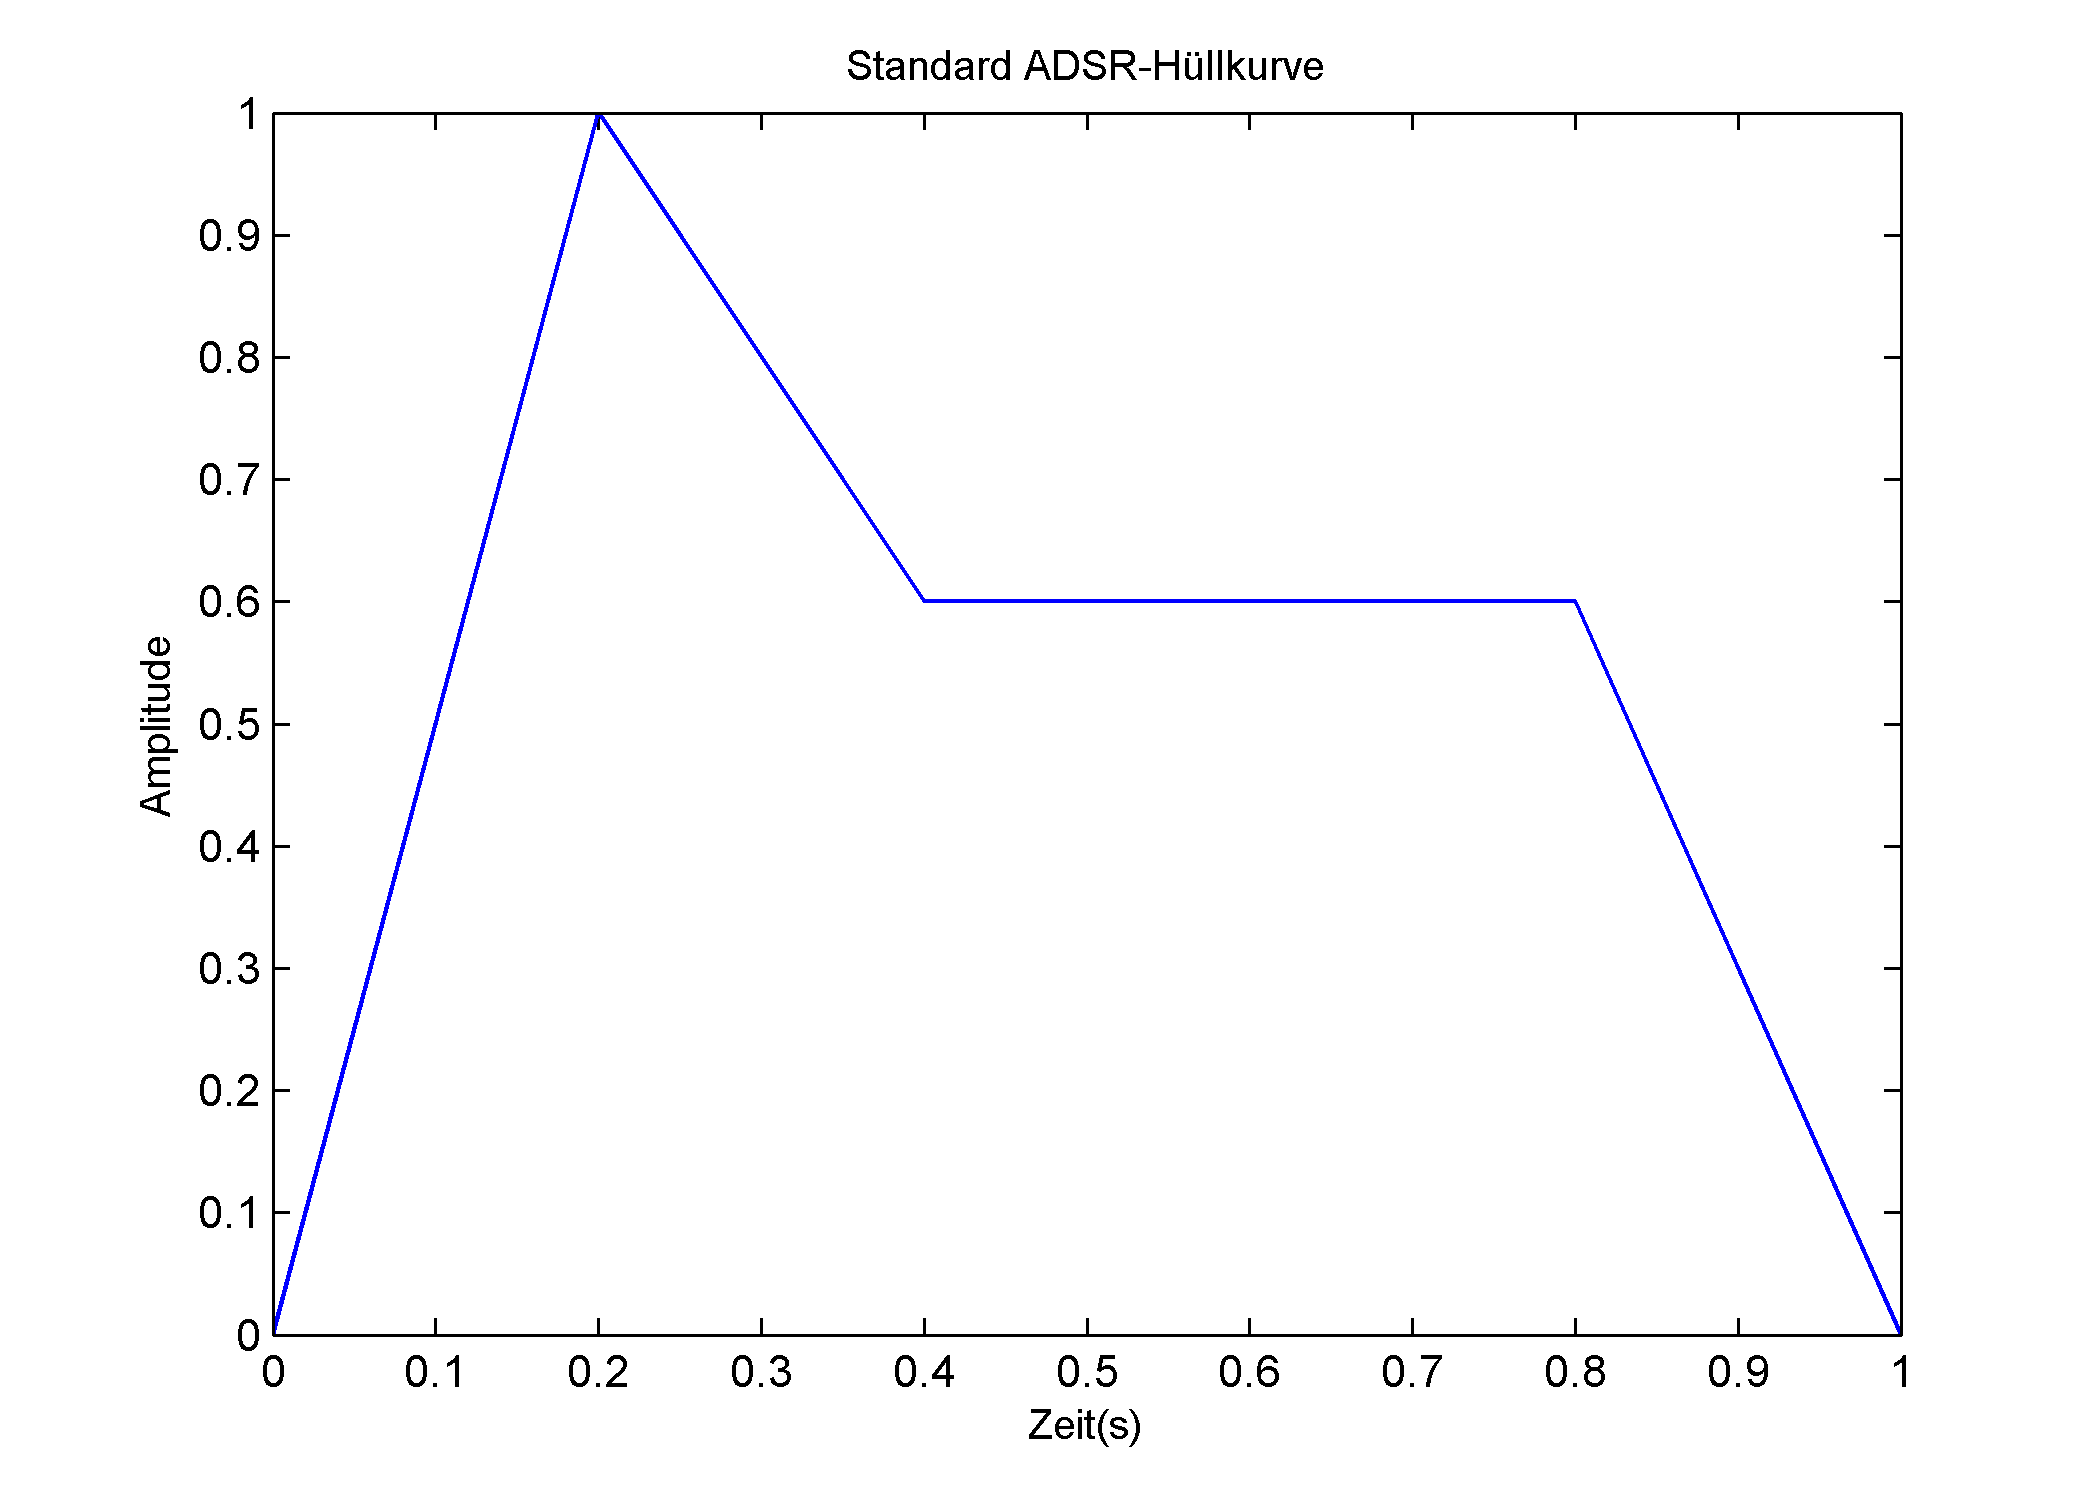
\includegraphics[width=0.5\textwidth]{adsrDefault.png}
\caption{Standard ADSR-Hüllkurve}
\label{fig:adsrDefault}
Quelle: Eigene Darstellung mit Matlab
\end{figure}

Da allerdings bei vielen Instrumenten die Lautstärke in den einzelnen Phasen der ADSR-Hüllkurve nicht gleichmäßig steigt oder sinkt, ist es nötig die Kurven beliebig Komplex abbilden zu können. Bei vielen Instrumenten steigt beispielsweise die Lautstärke in der Attack Phase exponentiell an und fällt in der Decay und Release Phase auch wieder exponentiell ab. Manche Synthesizer bieten zusätzlich auch noch eine Hold Phase vor der Attack Phase, da es Instrumente gibt, die einige Zeit benötigen bis sie nach dem Anschlagen des Tones in die Attack Phase eintreten. In Abbildung \ref{fig:adsrTypical} wurden weitere für Instrumenten typische Hüllkurven dargestellt um zu verdeutlichen, dass die ADSR-Hüllkurve bei Instrumenten beliebig komplexe Formen annehmen kann.

\begin{figure} [ht]
\centering
  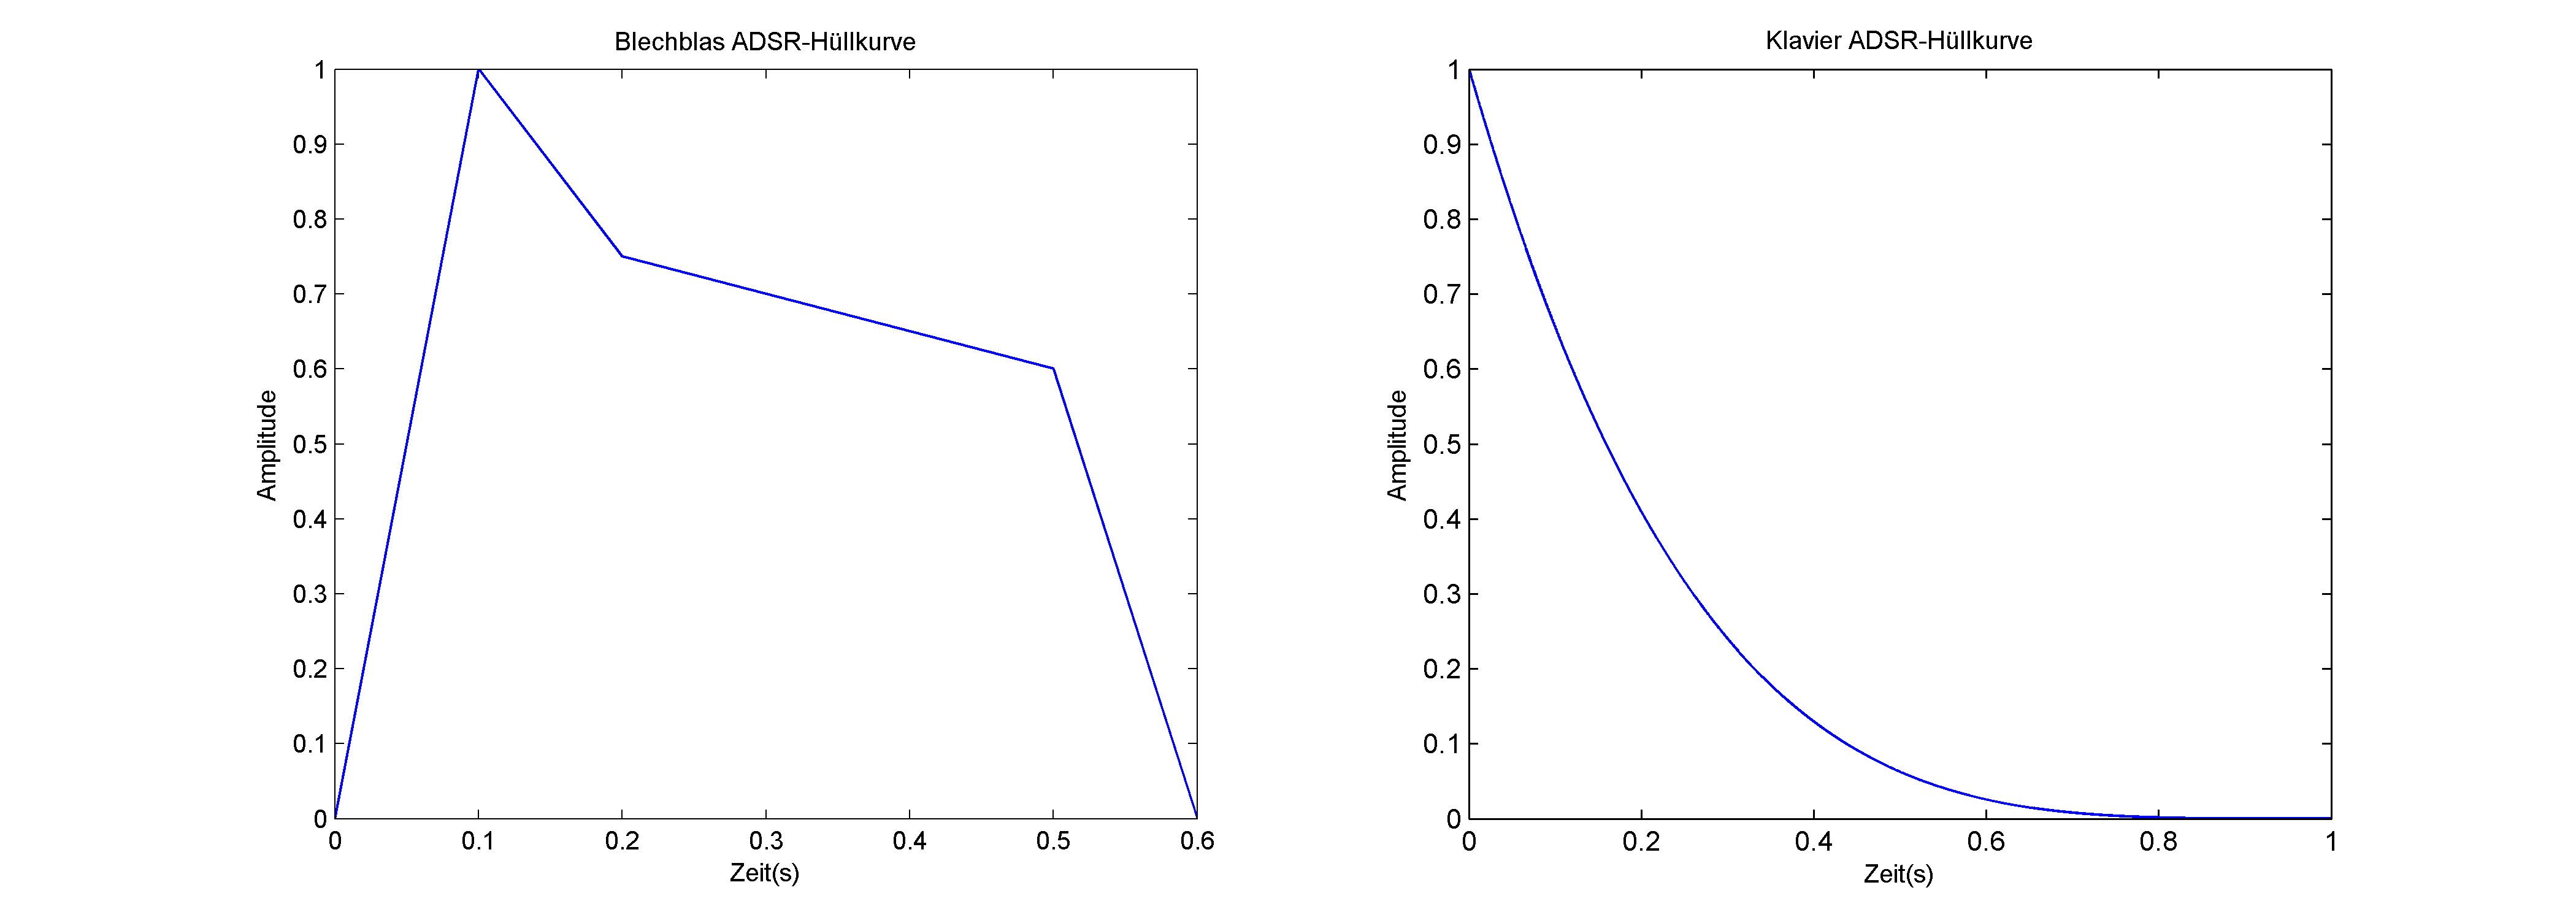
\includegraphics[width=1\textwidth]{adsrTypical.png}
\caption{Typische ADSR-Hüllkurve eines Blechblasinstrumentes und eines Klaviers}
\label{fig:adsrTypical}
Quelle: Eigene Darstellung mit Matlab
\end{figure}

Auch wenn das Hinzufügen einer ADSR-Hüllkurve den Klang des synthetisierten Tones schon natürlicher wirken lässt, hört sich der erzeugte Ton leider noch nicht wie ein echtes Instrument an. Eine weitere Möglichkeit ihn zu verbessern, stellt die Varrierung des Modulationsindex über die Zeit oder die Amplitude dar. Somit kann die Anzahl der Seitenfrequenzen verändert werden, was zu einem lebendigeren Klang führt. Bei Blasinstrumenten wird der Modulationsindex typischerweise über die Amplitude (also mit der ADSR-Hüllkurve) variiert. \cite[S. 532]{chowningPaper}

Eine weitere Möglichkeit den Klang des Tones zu verbessern stellen Filter dar. Filter können genutzt werden um das von der FM Synthese erzeugte Signal zu manipulieren. Dabei werden ungewollte Frequenzen gedämpft bzw. komplett heraus gefiltert. Typische Vertreter von Filtern sind Hochpassfilter, Tiefpassfilter, Bandpass und Bandsperre. \cite[S. 100-104]{stotz}

Das bisher erzeugte Signal ist noch ein reines Signal, welches so in der Natur nicht vorkommen kann. Bei Luftverwirblungen und Unebenheiten des Instrumentes tritt Rauschen auf. Dieses Rauschen trägt zum typischen Klangbild eines Instrumentes bei und sollte auch nachgebildet werden. Ein Rauschen kann mittels Feedback-FM-Synthese erzeugt werden, dafür muss der Modulationsindex der Feedback-FM-Synthese sehr hoch angesetzt werden. Das von der Feedback-FM-Synthese erzeugte Signal gleicht bei sehr hohem Modulationsindex einem weißen Rauschen. Anschließend kann dieses Rauschen mittels Multibandpassfilter um die jeweiligen ausgeprägten Frequenzen gefiltert werden. Würde das Rauschen nicht gefiltert werden, kann neben dem Ton, das Rauschen als solches wahrgenommen werden. [TODO CITE]

Um den Klang des Synthetisierten Tones noch natürlicher zu gestalten, könnte dem Ton noch ein Hall-Effekt hinzugefügt werden.


\FloatBarrier
\subsubsection{Nachbildung eines Tones einer Querflöte mittels FM-Synthese}

Im Laufe dieses Kapitels soll ein Ton einer Querflöte mittels FM-Synthese erzeugt und mit den oben beschriebenen Techniken verfeinert werden. Alle Beispiele sind in Matlab erstellt und können mit den beiliegenden Dateien nachgestellt werden. In Abbildung \ref{fig:plotFluteOrig} sind Spektrogram, Waveform und Spektrum des originalen Querflöten Tones abgebildet. Mit den Information aus den vorliegenden Grafiken wird versucht, diesen spezifischen Ton nachzubilden.

\begin{figure} [h!t!b!]
\centering
  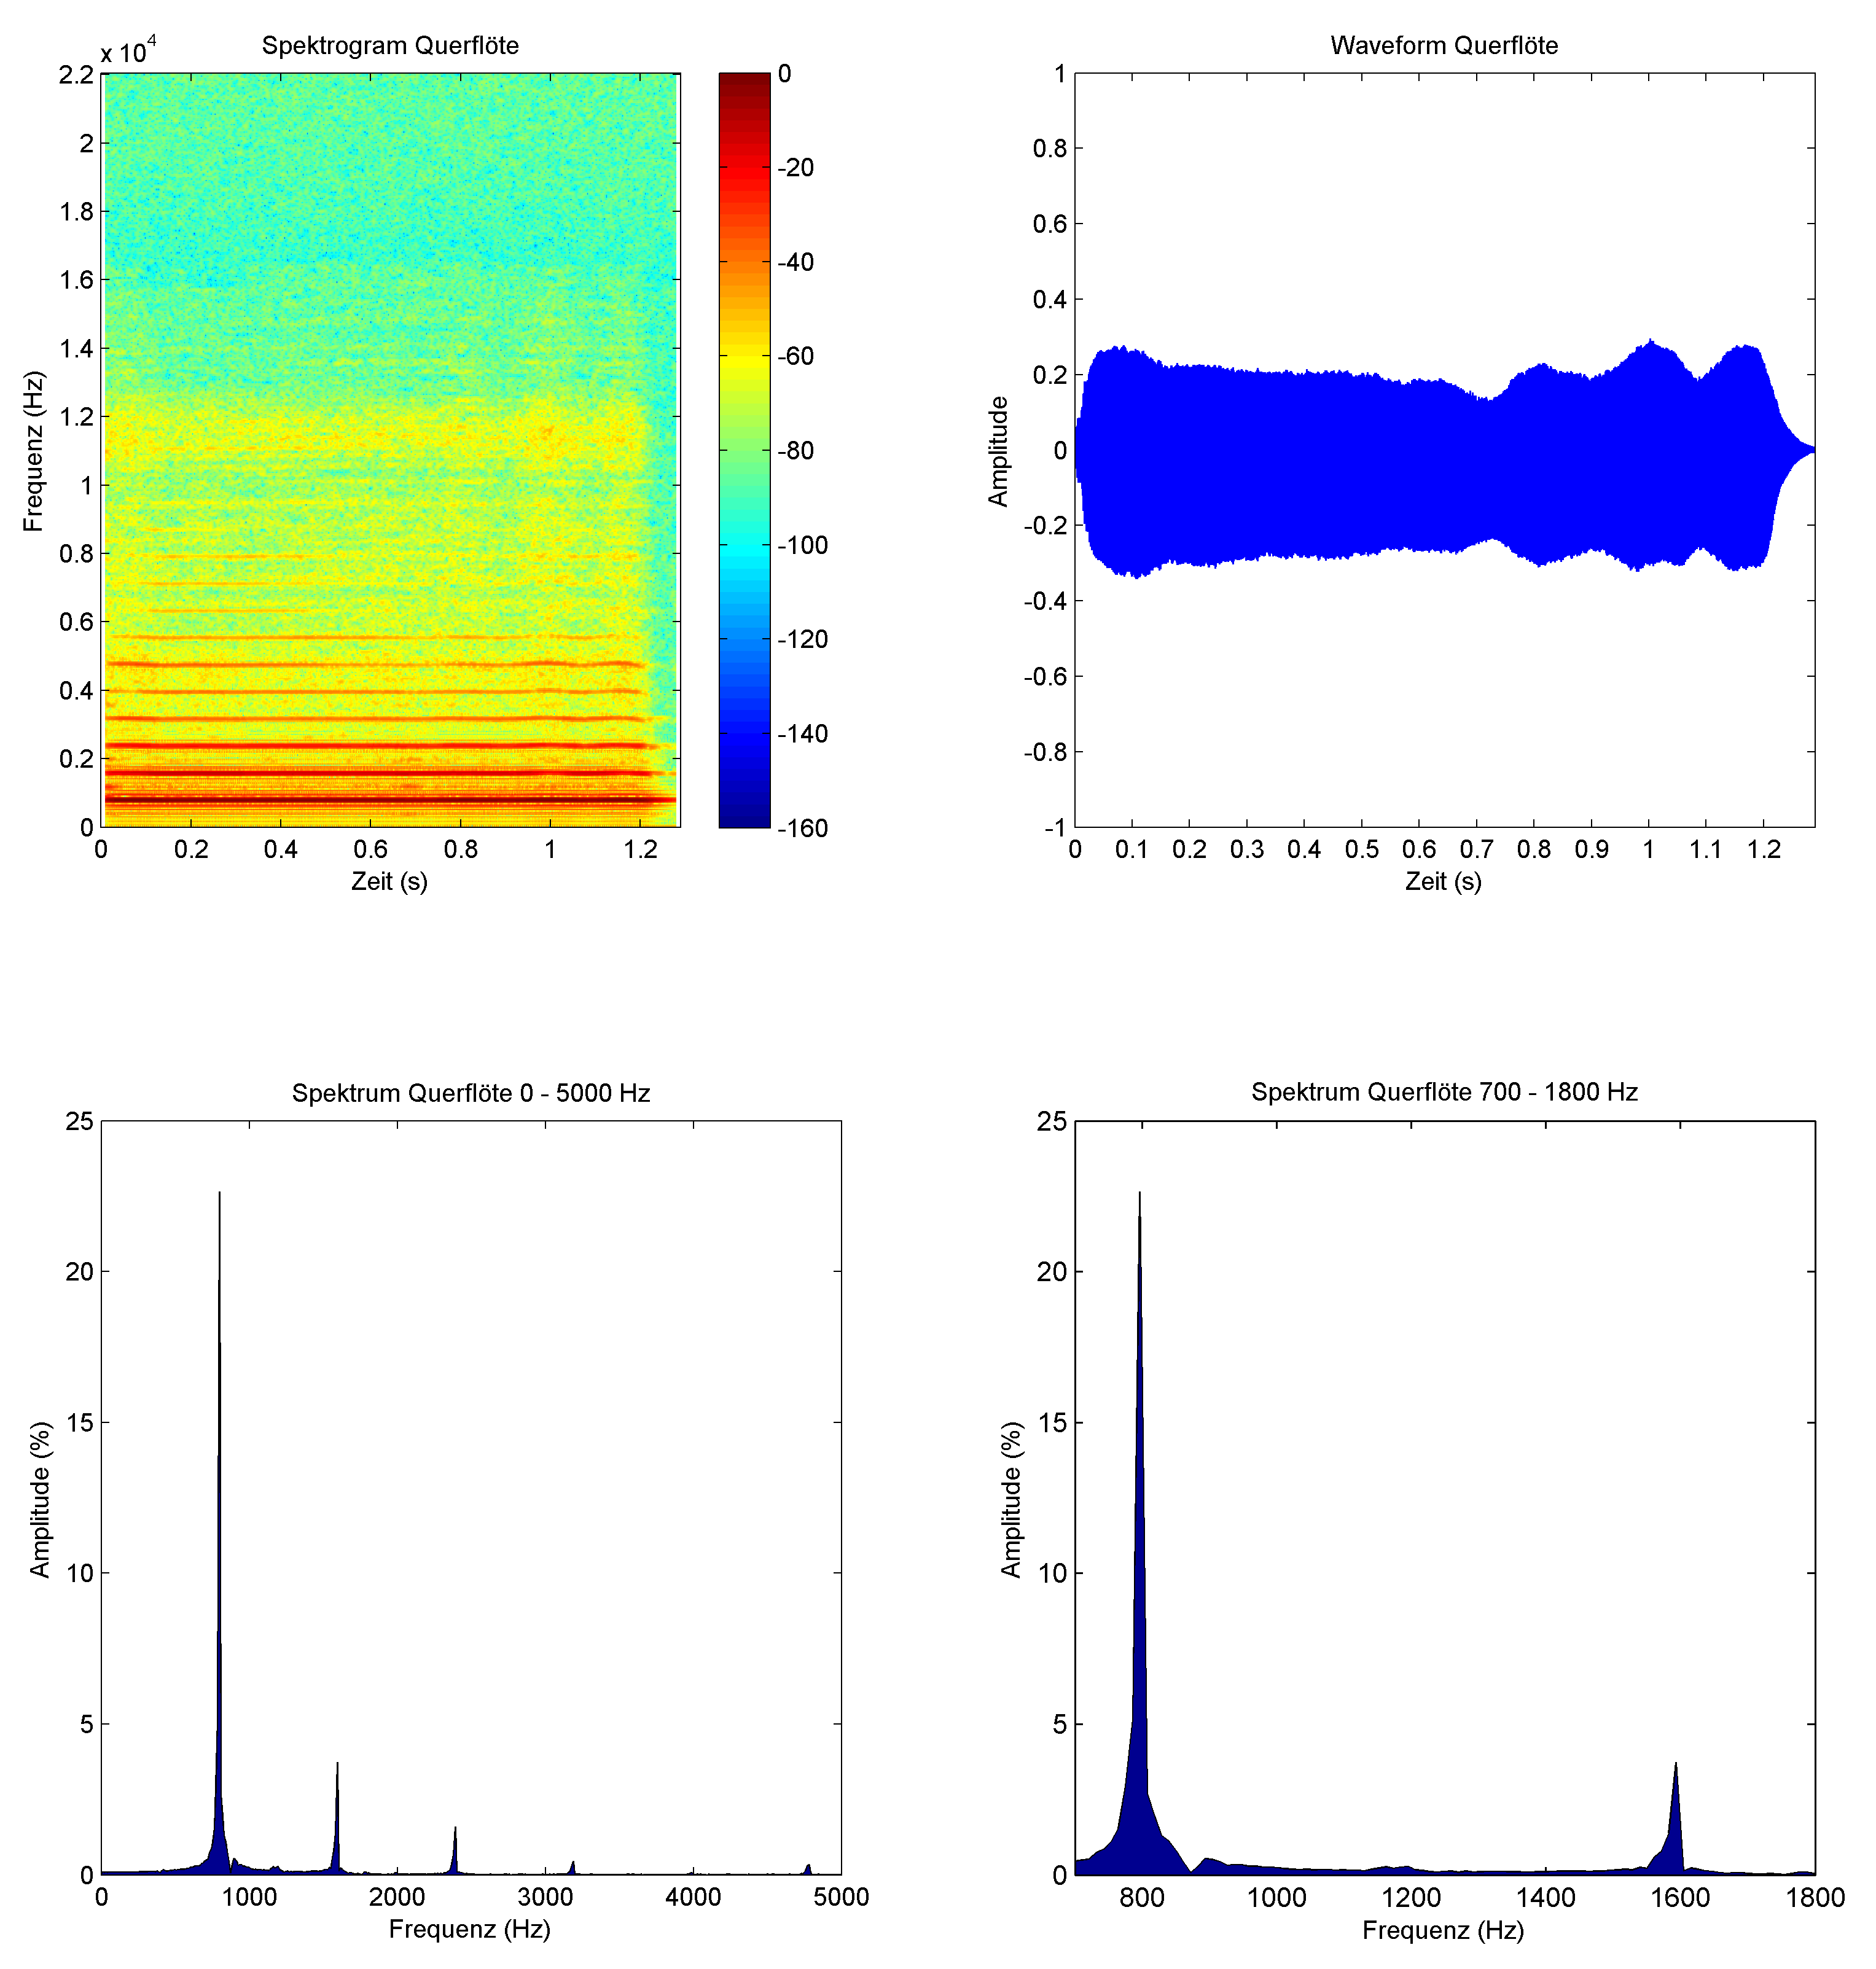
\includegraphics[width=1\textwidth]{plotFluteOrig.png}
\caption{Plot des Spektrograms, der Waveform und des Spektrums eines echten Tones einer Querflöte}
\label{fig:plotFluteOrig}
Quelle: Eigene Darstellung mit Matlab
\end{figure}

Anhand des Spektrums können bereits einige Erkenntnisse für die FM-Synthese ausgelesen werden. Zunächst ist zu bemerken, dass die am stärksten ausgeprägte Frequenz bei etwa 800 Hz liegt. Bei genauerer Betrachtung wird sichtbar, dass die Frequenz nicht exakt bei 800 Hz sondern bei 796.75 Hz ihren maximalen Ausschlag erreicht. Dies entspricht am ehesten einem G5 mit 784 Hz \cite[S. 181]{borucki}. Diese Frequenz (796.75 Hz) werden wir bei der FM-Synthese als Träger Frequenz nutzen. Im Spektrum sind außerdem noch mehrere Seitenfrequenzen zu sehen. Die erste dieser Seitenfrequenzen befindet sich bei etwa dem doppelten der Grundfrequenz. Bei genauerer Betrachtung wird sichtbar das sie ihren maximalen Amplitudenwert wirklich genau bei dem doppeltem der Grundfrequenz (1593.5 Hz) hat. Also ist der Abstand zwischen Grundfrequenz und erster Seitenfrequenz genauso groß wie der Abstand von 0 Hz bis zur Grundfrequenz, hierbei ist zu bemerken, dass der Abstand von einem ganzzahligen Multiplikator mit der Grundfrequenz typisch für einen harmonischen Ton ist \cite[S. 528]{chowningPaper}. Die nächsten Seitenfrequenzen haben jeweils wieder den selben Abstand von 796.75 Hz zur jeweiligen vorangegangenen Seitenfrequenz. Aus dieser Beobachtung können wir unsere Modulationsfrequenz von 796.75 Hz schließen. Anhand der Anzahl der sichtbaren Seitenfrequenzen im Spektrum können wir eine ungefähre Abschätzung unseres Modulationsindexes wagen. Somit wird als Modulationsindex für die ersten Tests vorerst 0.5 angenommen. 

\begin{figure} [ht]
\centering
  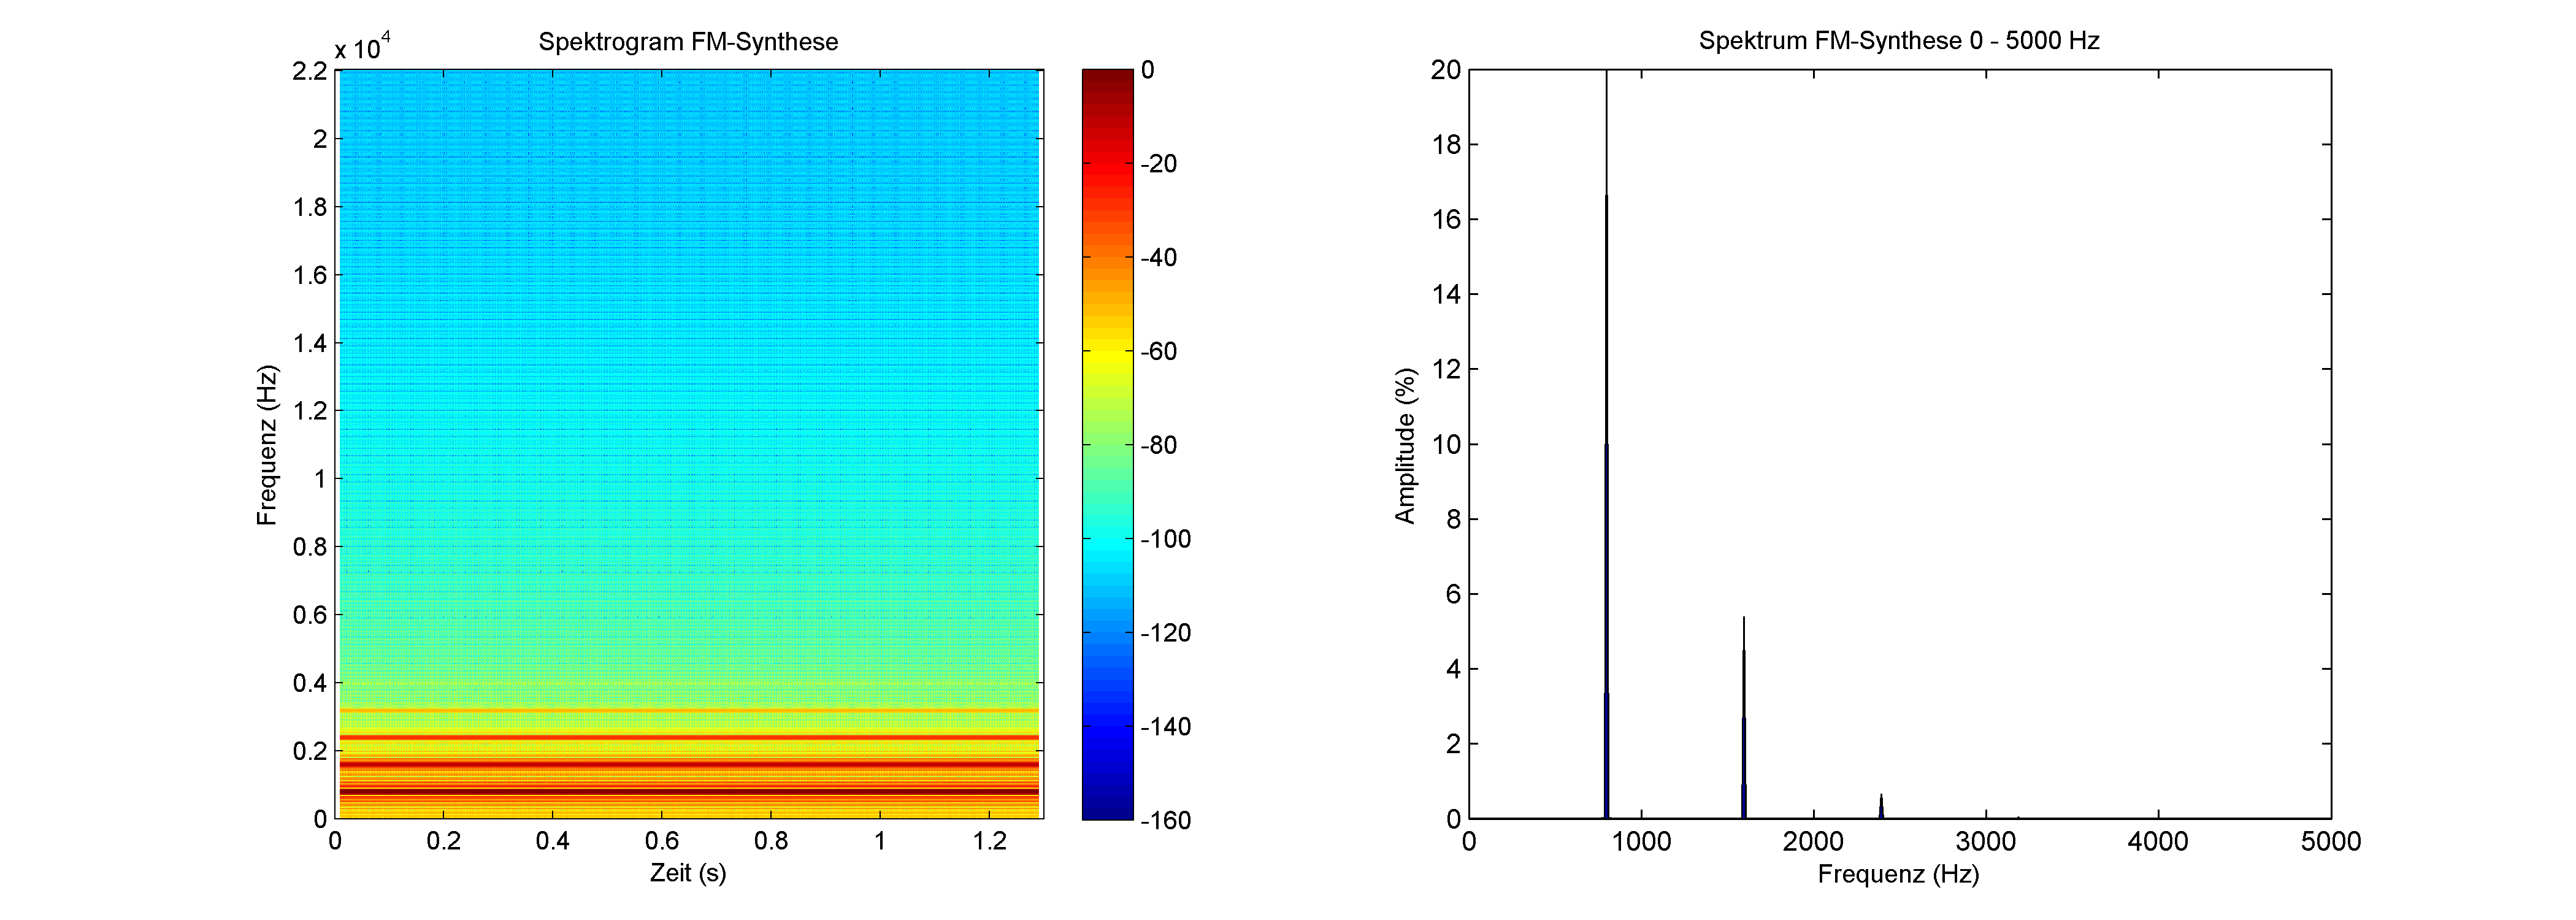
\includegraphics[width=1\textwidth]{plotFMSyntheseI05.png}
\caption{Plot des Spektrograms und des Spektrums der FM-Synthese mit den Parametern fc = 796.75 Hz, fm = fc und I = 0.5 }
\label{fig:plotFMSyntheseI05}
Quelle: Eigene Darstellung mit Matlab
\end{figure}

Ein erstes Spektrum der FM-Synthese mit den eben festgelegten Werten kann in Abbildung \ref{fig:plotFMSyntheseI05} begutachtet werden. Beim Evaluieren der Ergebnisse dieses Spektrums fällt auf, dass die erste Seitenfrequenz im Verhältnis zur Grundfrequenz einen viel Stärkeren Ausschlag aufweist als es bei der Querflöte der Fall ist. Außerdem fällt danach die Amplitude der 2. und 3. Seitenfrequenz viel stärker ab als bei dem Instrument. Sieht man sich jetzt noch das Spektrogram (ebenfalls in Abbildung \ref{fig:plotFMSyntheseI05}) an, fällt im Vergleich zum Spektrogram der Querflöte die sehr viel geringer Anzahl an Seitenfrequenzen auf. Die Seitenfrequenzen bei 4000 Hz und darüber sind bei dem Instrument noch deutlich sichtbar während sie bei der FM-Synthese schon bei 4000 Hz kaum noch existent sind. Versucht man jetzt den Modulationsindex zu erhöhen um die Anzahl der Seitenfrequenzen zu erhöhen, verlagert sich die Amplitude unserer Trägerfrequenz auf die Seitenfrequenzen, damit werden die Seitenfrequenz stärker und die Träger Frequenz schwächer, zu sehen in Abbildung \ref{fig:spektrumFMSyntheseI2}. 

\begin{figure} [ht]
\centering
  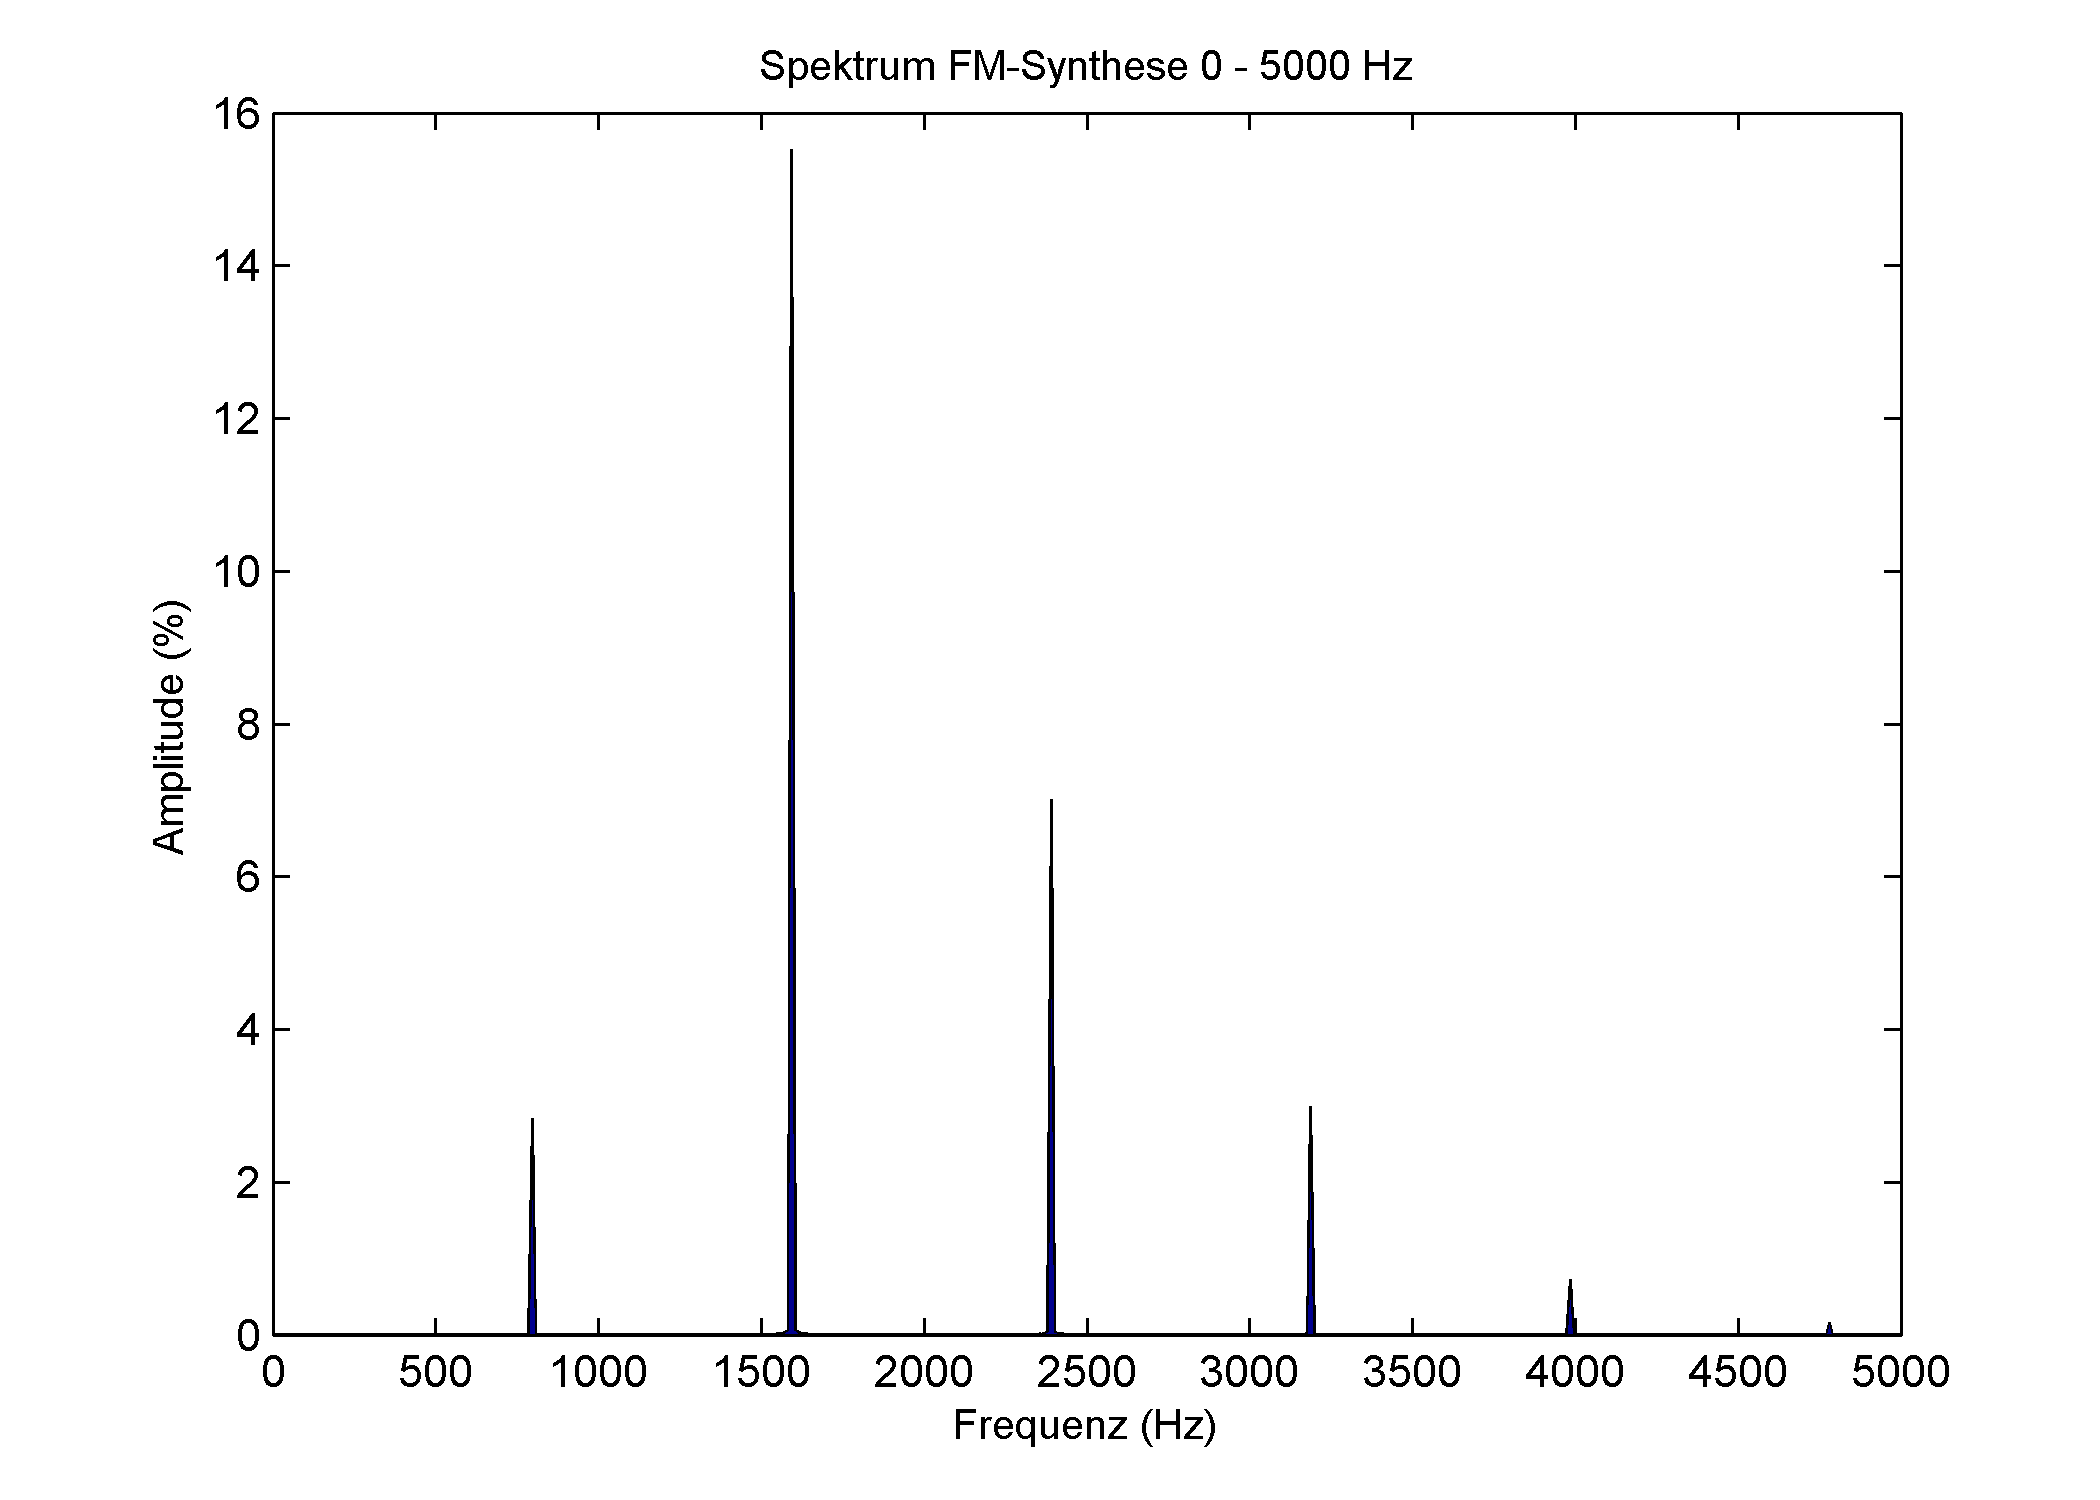
\includegraphics[width=0.5\textwidth]{spektrumFMSyntheseI2.png}
\caption{Plot des Spektrums der FM-Synthese mit den Parametern fc = 796.75 Hz, fm = fc und I = 2}
\label{fig:spektrumFMSyntheseI2}
Quelle: Eigene Darstellung mit Matlab
\end{figure}

Um dieses Verhalten zu umgehen müssen wir uns der Komplexen FM-Synthese widmen. Hier werden mehrere Modulatoren verschachtelt um eine größere Anzahl an Seitenfrequenzen zu erzeugen. Allerdings ist es bei der Komplexen FM-Synthese schwer vorauszusagen wie stark die Amplituden der einzelnen Seitenfrequenzen ausgeprägt sind, deshalb braucht es hier einige Experimente um auf das gewünschte Ergebnis zu stoßen. In Abbildung \ref{fig:plotFMSyntheseKomplex4Mod} sehen sie das Ergebnis der FM-Synthese mit 4 Modulatoren. Dieses Spektrum ähnelt dem der Querflöte schon sehr viel stärker und auch das Spektrogram weißt in den Intensitäten der Seitenfrequenzen eine deutliche Ähnlichkeit auf.

\begin{figure} [ht]
\centering
  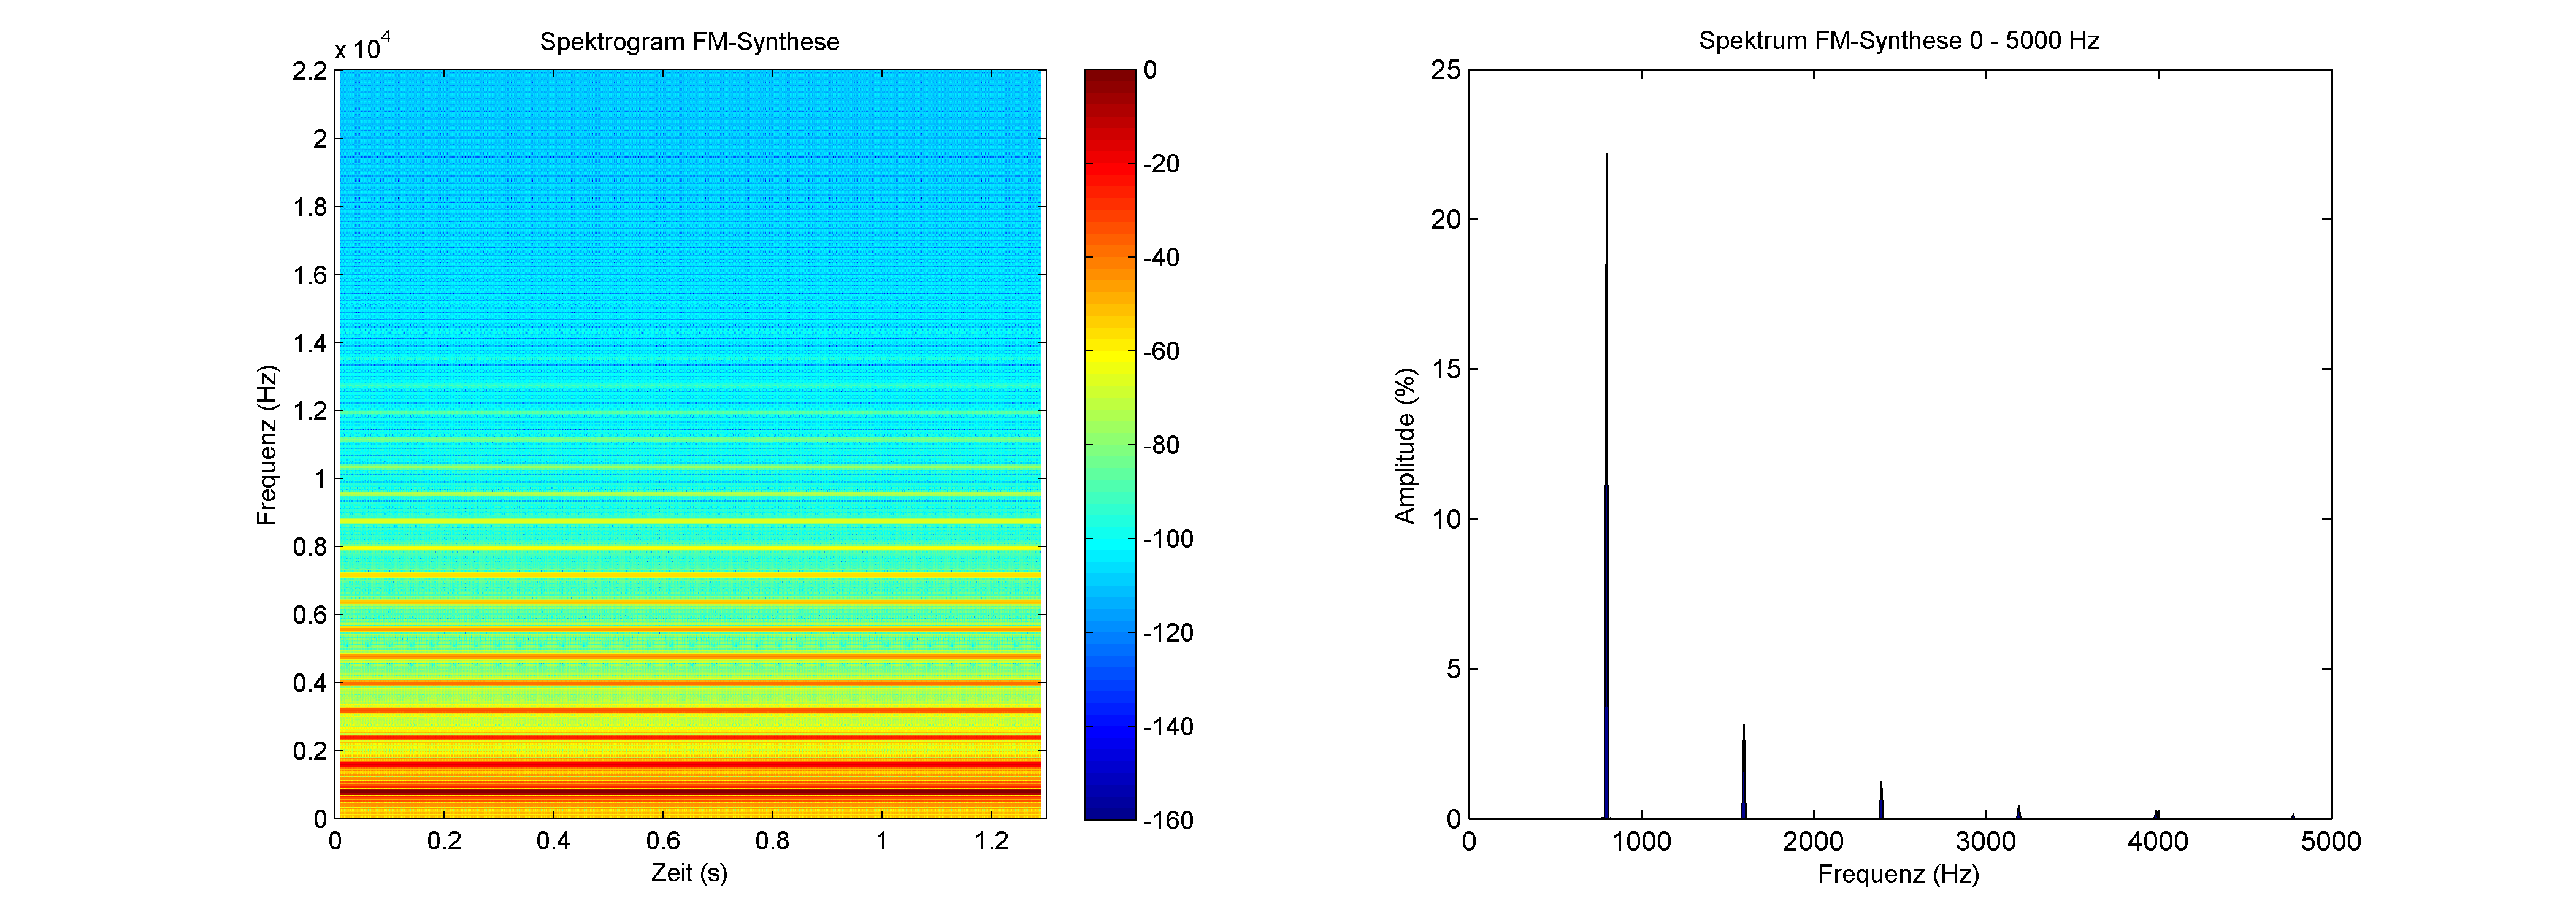
\includegraphics[width=1\textwidth]{plotFMSyntheseKomplex4Mod.png}
\caption{Plot des Spektrograms und des Spektrums der FM-Synthese mit 4 Modulatoren und den Parametern fc = 796.75 Hz, fm1 = fm2 = fm3 = fm4 = fc, I1 = 0.3, I2 = 0.5, I3 = 1 und I4 = 1}
\label{fig:plotFMSyntheseKomplex4Mod}
Quelle: Eigene Darstellung mit Matlab
\end{figure}

Da die Grundeinstellung der FM-Synthese mit den oben genannten Parametern ein zufriedenstellendes Signal erzeugt, können wir uns jetzt der Veredlung des Tones widmen. Zuerst wird dem Signal ein Vibrato hinzugefügt. Durch das Hinzufügen des Vibratos, schwingt der erzeugte Ton leicht und wirkt lebendiger und nicht ganz so künstlich. Dies kann bewerkstelligt werden indem die Modulationsfrequenz leicht erhöht oder verringert wird. Auch hierbei muss experimentiert werden, welche Erhöhung der Modulationsfrequenz das gewünschte Ergebnis erzeugt. Als sehr ähnlich zum Original Ton hat sich in diesem Fall eine Erhöhung um 2.5 Hz herausgestellt. Unsere neue Modulationsfrequenz ist somit fm = fc + 2.5. In Abbildung \ref{fig:spektrumFMSyntheseVibrato} wird die Auswirkung des Vibratos sichtbar, es bilden sich um die Seitenfrequenzen weitere recht gering ausgeprägte Frequenzausschläge.

\begin{figure} [ht]
\centering
  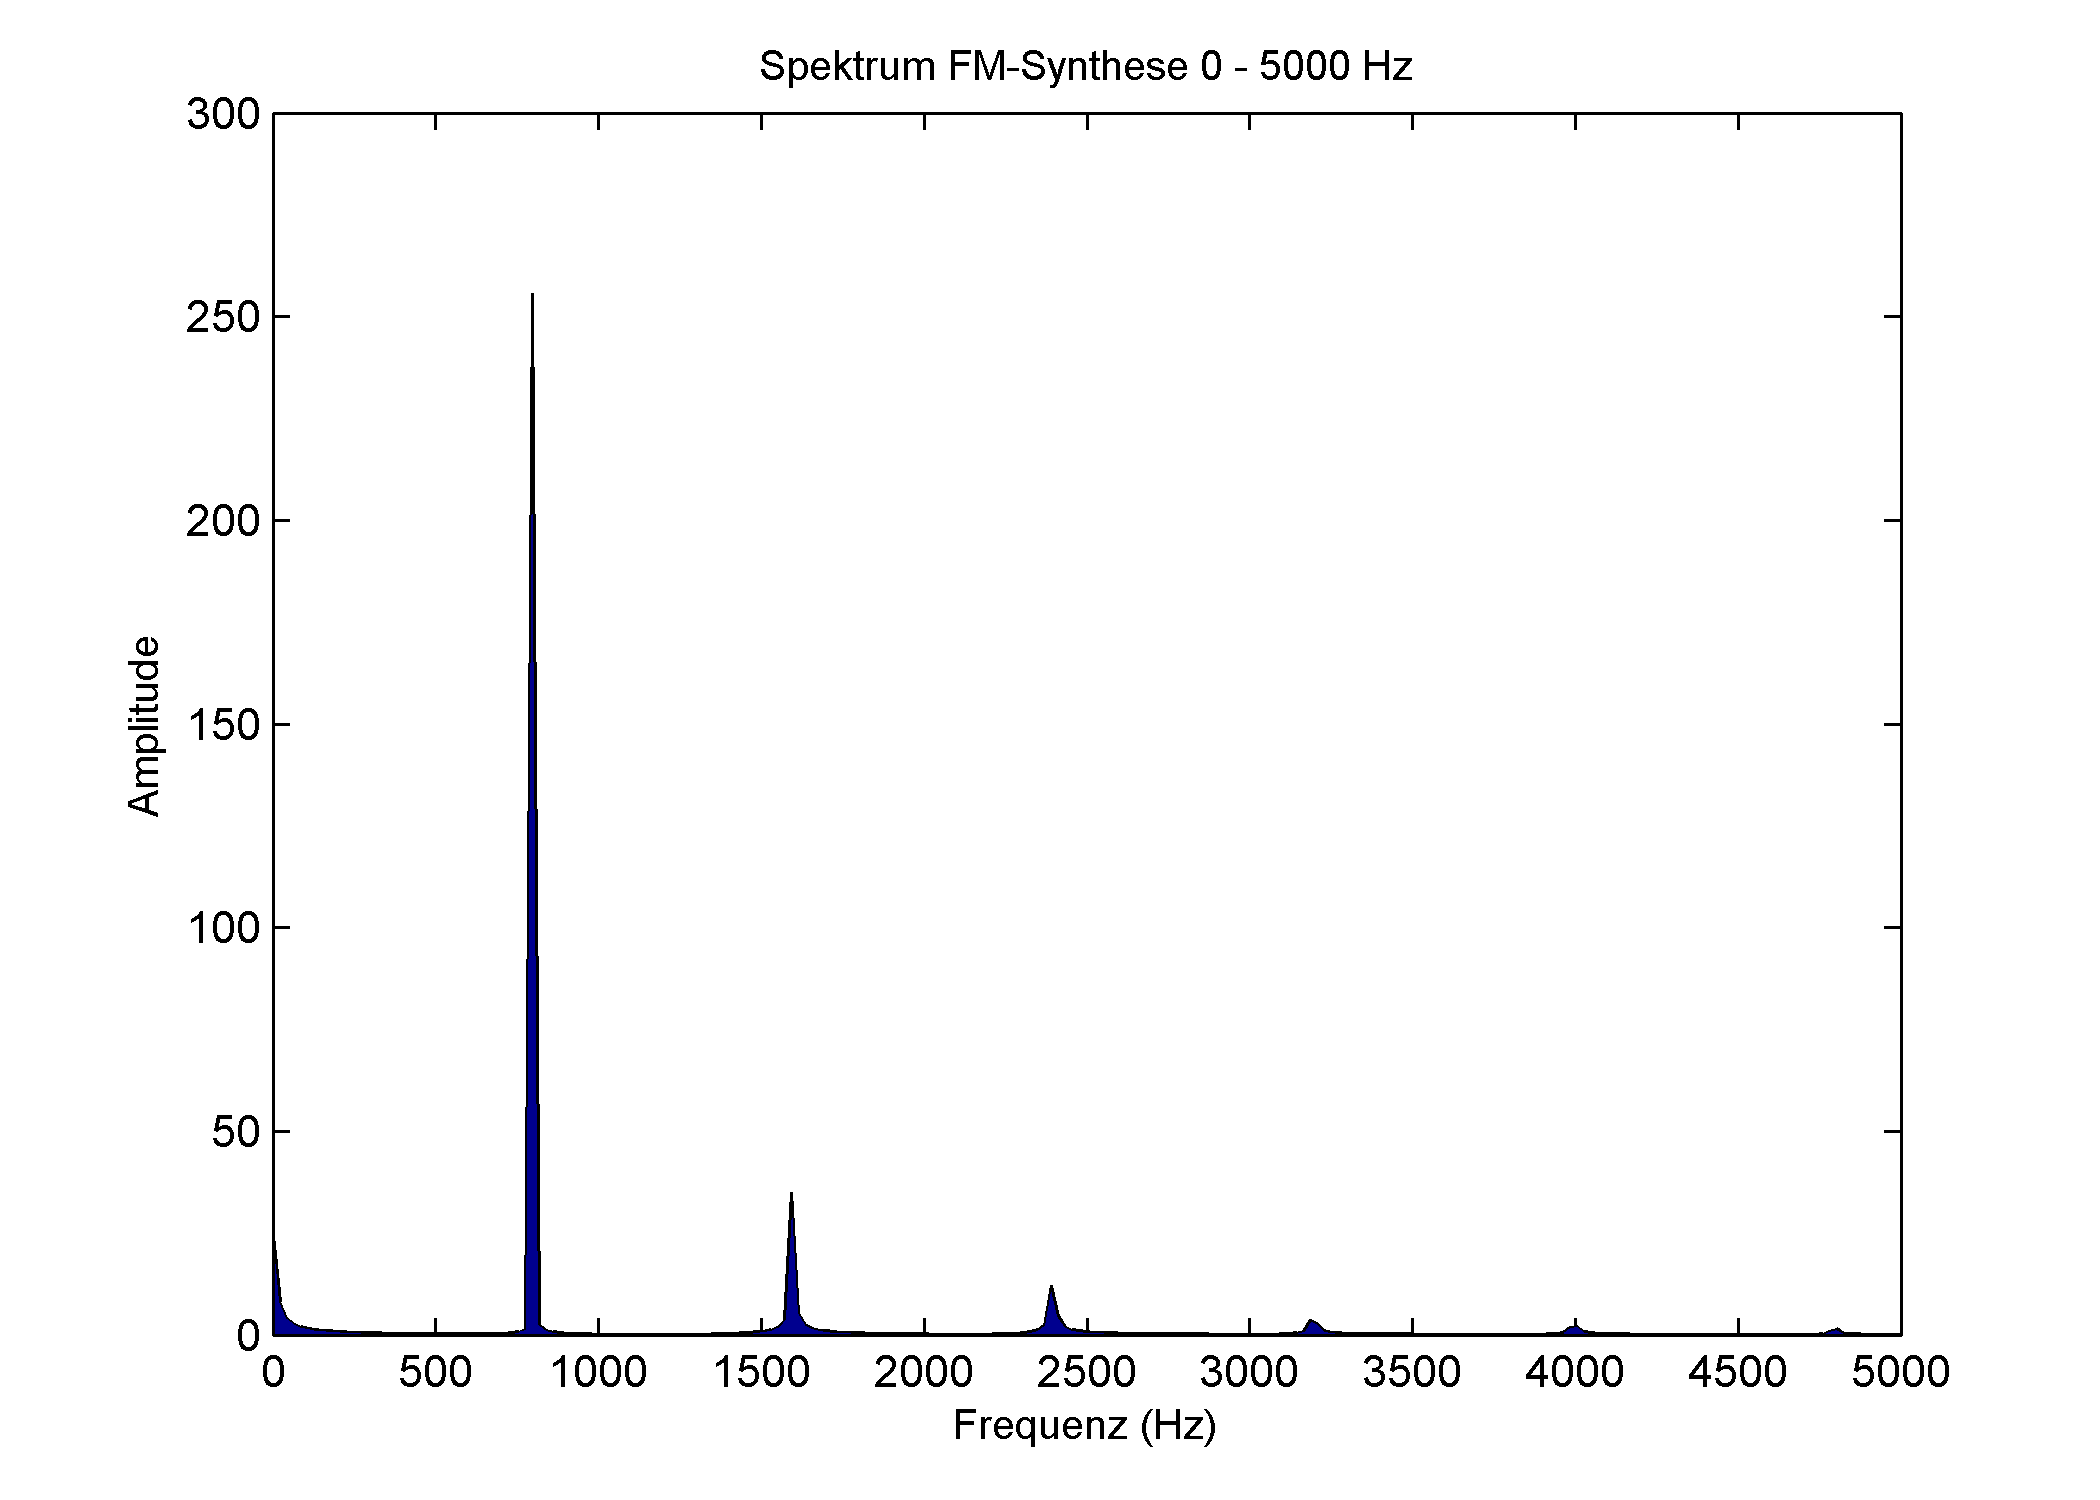
\includegraphics[width=0.5\textwidth]{spektrumFMSyntheseVibrato.png}
\caption{Plot des Spektrums der FM-Synthese mit 4 Modulatoren, Vibrato und den Parameter fc = 796.75 Hz, fm1 = fm2 = fm3 = fm4 = fc +2.5, I1 = 0.3, I2 = 0.5, I3 = 1 und I4 = 1}
\label{fig:spektrumFMSyntheseVibrato}
Quelle: Eigene Darstellung mit Matlab
\end{figure}

Der nächste wichtige und einfach hinzuzufügende Bestandteil des synthetisierten Tones ist die ADSR-Hüllkurve. Um generell eine Querflöte nachzumachen wäre eine Hüllkurve wie in Abbildung \ref{fig:adsrFlute} links gezeigt möglich. Allerdings versuchen wir den originalen Ton der Querflöte so gut wie möglich nachzuahmen, hierfür wurde eine Komplexere Hüllkurve nach dem Beispiel der Waveform des original Tones generiert. Bei dieser Hüllkurve wurde Attack, Decay und Release von der Allgemeinen Hüllkurve übernommen und die Sustain Phase angepasst, zu sehen in Abbildung \ref{fig:adsrFlute} rechts. 

\begin{figure} [ht]
\centering
  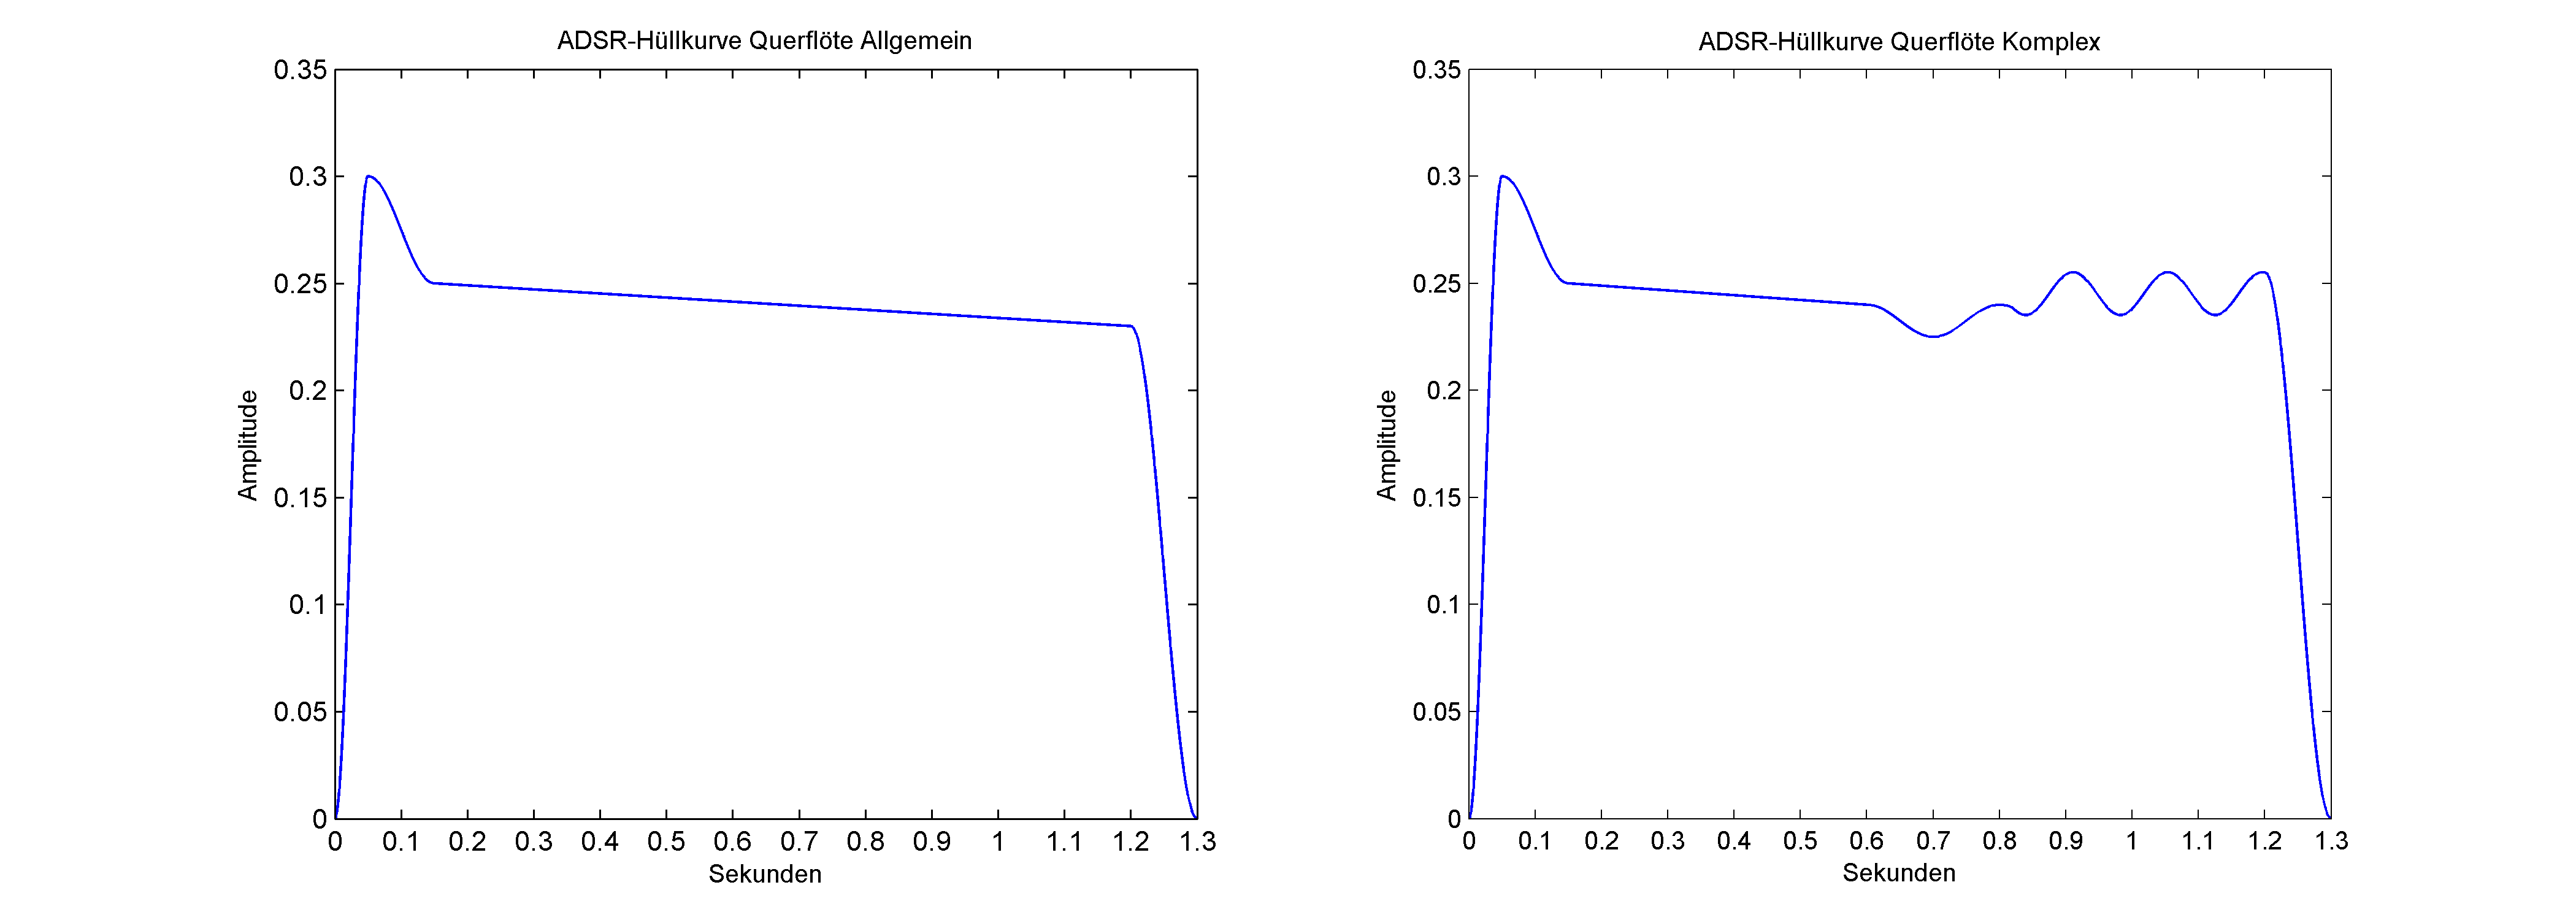
\includegraphics[width=1\textwidth]{adsrFlute.png}
\caption{Plot der ADSR-Hüllkurve einer Querflöte und der hier genutzten, komplexeren Hüllkurve}
\label{fig:adsrFlute}
Quelle: Eigene Darstellung mit Matlab
\end{figure}

Nachdem die ADSR-Hüllkurve hinzugefügt wurde, fällt im Spektrogram auf, dass die Seitenfrequenzen trotz geringerer Amplitude bei Attack und Release Phase einen größeren Ausschlag als beim Instrument aufweist. Dieser Ausschlag kann verringert werden, indem der erste Modulationsindex mit der ADSR-Hüllkurve variiert wird. 

Nachdem Vibrato, Variabler Modulationsindex und ADSR-Hüllkurve hinzugefügt wurden, hat sich das Spektrogram zur Abbildung \ref{fig:plotFMSyntheseKomplex4Mod} kaum geändert. Es wird nur der Vibrato durch die etwas breiteren Seitenfrequenzen und die ADSR-Hüllkurve durch ansteigen des Spektrums zu Beginn des Tones und Abfallen des Spektrums nach 1.2 Sekunden sichtbar. Der Ton hört sich von der Tonhöhe und der Intensität schon stark nach dem Originalen Querflötenton an. Allerdings fehlen noch die Typischen Blas- und Luftverwirblungsgeräusche sowie das sehr starke Anblasgeräusch. Um die typischen Blasgeräusche zu erzeugen wird zunächst ein Rauschen mittels FM Feedback Generator mit hohem Modulationsindex erzeugt. Würde das Rauschen ohne weitere Arbeitsschritte dem synthetisiertem Signal hinzugefügt, könnte das Rauschen stark herausgehört werden. Um dies zu verhindern muss das Rauschen vorerst gefiltert werden. Hierzu wird ein Multibandpassfilter über alle möglichen Seitenfrequenzen erstellt. Das Gefilterte Rauschen wird anschließend noch mit einer ADSR-Hüllkurve veredelt. Dieser Schritt ist nötig, da während der Attack-Phase des Original Tones, wie im Spektrogram in Abbildung \ref{fig:plotFluteOrig} zu sehen, das Rauschen durch das Anblasen des Instrumentes sehr scharf heraus sticht. Zusätzlich kann noch ein sehr leises Rauschen des Feedback-FM-Generators ohne Filter über das ganze Frequenzspektrum gelegt werden um auch in den höheren Frequenzen einen leichten Ausschlag im Spektrogram kenntlich zu machen. Trotz des verstärkten Rauschens zu Begin des Tones, fehlt noch der Starke hörbare Ton der dabei entsteht. Beim betrachten des Spektrums und des Spektrograms fallen noch 2 recht Starke Ausschläge zu Begin des Signals auf. Ein Ausschlag befindet sich bei 904.3 Hz und der zweite bei 1182 Hz. Beide Frequenzen können mit einem einfachen Sinus erzeugt und mit einer ADSR-Hüllkurve, die nur eine kurze Attack-Phase aufweist, modeliert und zum Signal addiert werden. In Abbildung \ref{fig:spektrogramFMSyntheseComplete} ist das Ergebnis der FM-Synthese mit den, in diesem Kapitel, besprochenen Veredelungen gezeigt. In den Plots sind die Ähnlichkeiten zum originalen Ton deutlich zu sehen.

\begin{figure} [h!t!b!]
\centering
  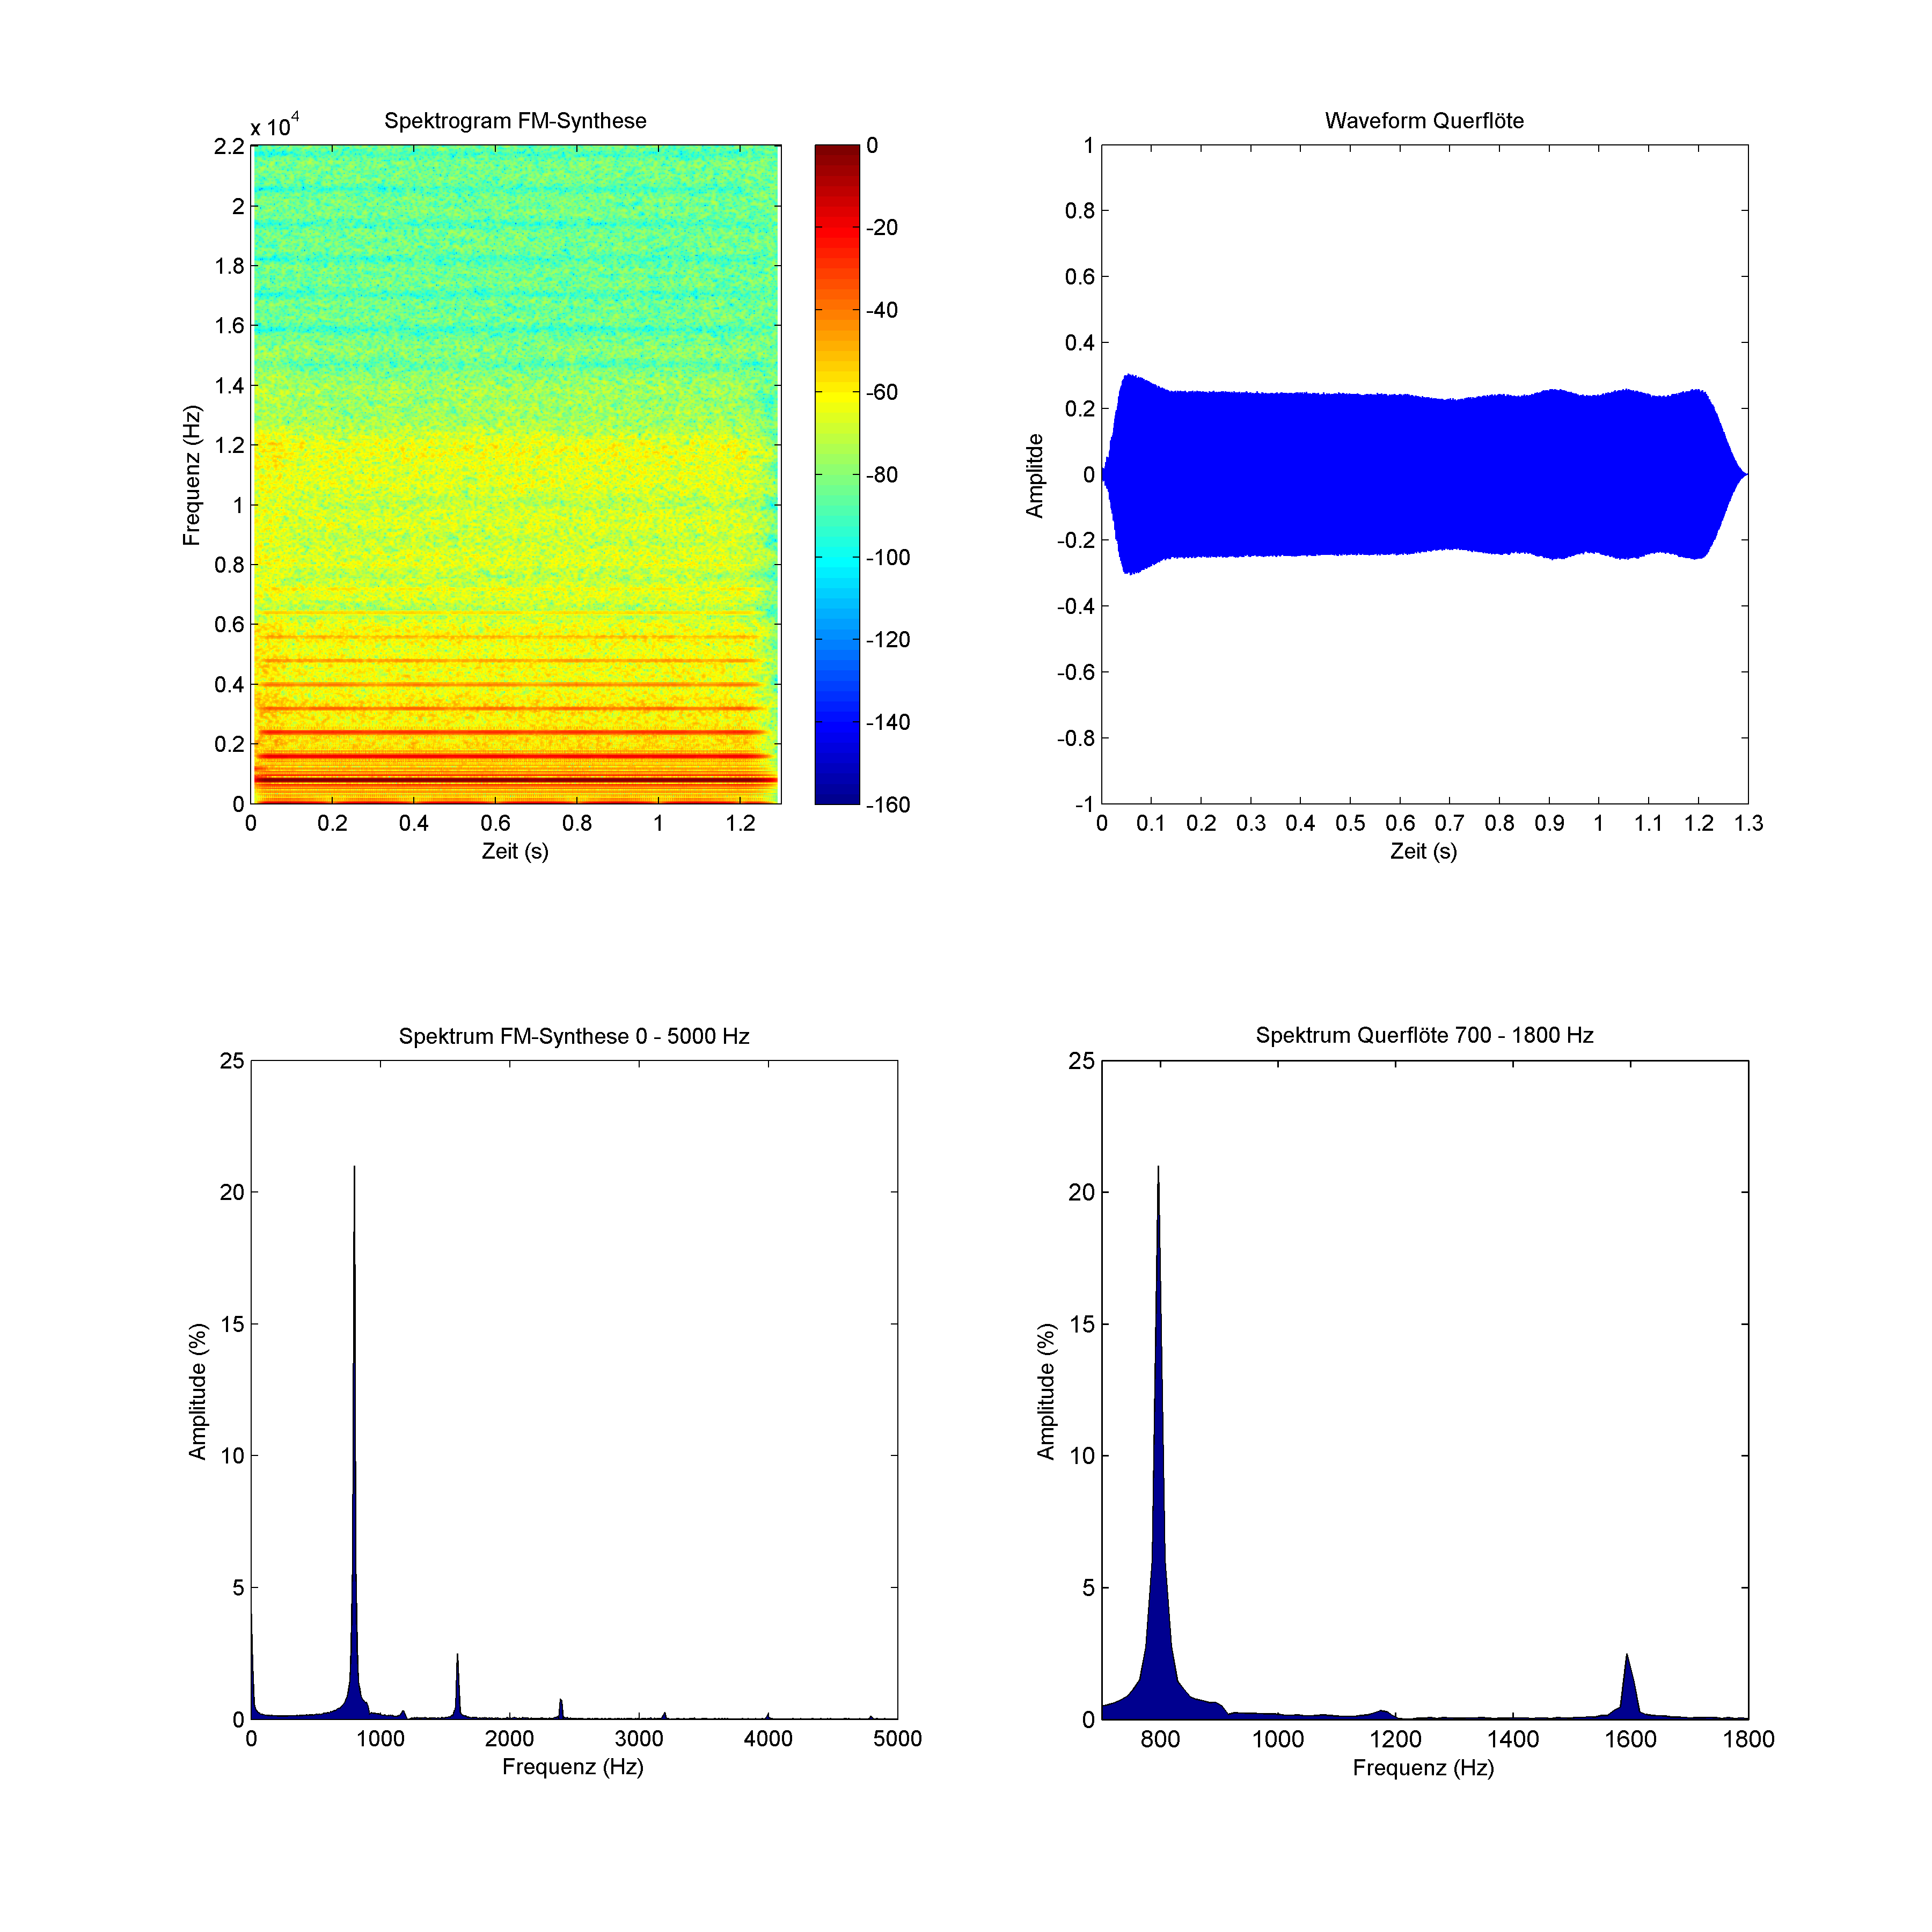
\includegraphics[width=1\textwidth]{spektrogramFMSyntheseComplete.png}
\caption{Plot des fertigen Tones der FM-Synthese mit 4 Modulatoren, ADSR-Hüllkurve, Variablem Modulationsindex, Vibrato, Rauschen und Anblasgeräusch}
\label{fig:spektrogramFMSyntheseComplete}
Quelle: Eigene Darstellung mit Matlab
\end{figure}

Der in diesem Kapitel synthetisierte Ton gleicht dem originalen Flöten Ton sehr stark. Trotzdem weißt der Flöten Ton noch etwas mehr Lebendigkeit auf, da das gesamte Signal nicht so statisch wie das, der FM-Synthese ist. 

Dieses Ergebnis zeigt, dass es sehr wohl möglich ist, wenn auch mit erheblichem Aufwand verbunden, mit der FM-Synthese einen natürlich wirkenden Instrumententon zu erzeugen. Gerade in diesem Beispiel fällt allerdings auf das der synthetisierte Ton im Vergleich zum originalen Ton nicht ganz so lebendig empfunden wird. Das hängt in diesem Fall vorallem an der nicht sehr neutralen Spielweise des Querflötenspielers.


\FloatBarrier
\subsubsection{FM Parametrisierung mittels Genetischer Algorithmen}

Mittels genetischer Algorithmen ist es möglich Parameter der FM Synthese herauszufinden, die nötig sind um einen Ton zu erzeugen der einem echten Instrument nachempfunden ist. Diese Algorithmen zerlegen einen echten Ton eines Instrumentes mittels Schneller Fourier Transformation in seine einzelnen Bestandteile und versucht verschiedene Parameter für die Synthese aus, zerlegt das entstandene Signal wieder mittels Schneller Fourier Transformation und vergleicht die Ergebnisse. Mit diesem Verfahren können recht zuverlässig realistisch Synthetisierte Töne erzeugt werden, die von einem Originalen Instrument kaum zu unterscheiden sind. Da für die Implementierung eines solchen Algorithmus allerdings die Zeit fehlt, wird dieses Thema in dieser Arbeit nicht weiter vertieft. Eine Ausführliche Erklärung der FM Parametrisierung mittels Genetischer Algorithmen kann in Andrew Horners Artikel "Nested Modulator and Feedback FM Matching of Instrument Tones" nachgelesen werden.

\FloatBarrier
\subsection{Modulationsframework (Theorie -> Praxis)}
\FloatBarrier
\subsection{Demo: Parameter und Effekte - Grafiken (evtl. Plotten)}